\documentclass[11pt,letterpaper]{article}

% ============================================================================
% PACKAGES
% ============================================================================
\usepackage[utf8]{inputenc}
\usepackage[T1]{fontenc}
\usepackage{helvet}
\renewcommand{\familydefault}{\sfdefault}
\usepackage[margin=0.85in, headheight=28pt]{geometry}
\usepackage{graphicx}
\usepackage{xcolor}
\usepackage{tikz}
\usepackage{tcolorbox}
\usepackage{booktabs}
\usepackage{enumitem}
\usepackage{hyperref}
\usepackage{fancyhdr}
\usepackage{titlesec}
\usepackage{multicol}
\usepackage{listings}
\usepackage{upquote}
\usepackage{amsmath,amssymb}
\usepackage{pgfplots}
\usepackage{array}
\usepackage{longtable}

% Ragged-right paragraph columns to prevent word spacing issues
\newcolumntype{L}[1]{>{\raggedright\arraybackslash}p{#1}}

% Increase vertical spacing between table rows for readability
\renewcommand{\arraystretch}{1.4}
\usepackage{colortbl}
\usepackage{pifont}
\usepackage{setspace}
\usepackage{parskip}
\usepackage{caption}
\usepackage{tabularx}

\pgfplotsset{compat=1.18}
\usetikzlibrary{shapes.geometric, arrows.meta, positioning, calc, decorations.pathreplacing, backgrounds, fit, shadows.blur, matrix, patterns, fadings, shadings}

% ============================================================================
% COLOR DEFINITIONS - Institutional Research Theme
% ============================================================================
\definecolor{instdark}{HTML}{1C2833}
\definecolor{instnavy}{HTML}{2C3E50}
\definecolor{instblue}{HTML}{34495E}
\definecolor{instaccent}{HTML}{5D6D7E}
\definecolor{instgold}{HTML}{B7950B}
\definecolor{instslate}{HTML}{566573}
\definecolor{successgreen}{HTML}{1E8449}
\definecolor{warningamber}{HTML}{B9770E}
\definecolor{alertcoral}{HTML}{922B21}
\definecolor{infocyan}{HTML}{1A5276}
\definecolor{coolgray}{HTML}{7B7D7D}
\definecolor{lightgray}{HTML}{EAECEE}
\definecolor{codebg}{HTML}{F4F6F7}
\definecolor{codetext}{HTML}{2C3E50}
\definecolor{gridlight}{HTML}{D5D8DC}
\definecolor{nodecyan}{HTML}{2E86AB}
\definecolor{nodeorange}{HTML}{D35400}
\definecolor{nodegreen}{HTML}{27AE60}
\definecolor{nodepurple}{HTML}{8E44AD}

% ============================================================================
% HYPERREF SETUP
% ============================================================================
\hypersetup{
  colorlinks=true,
  linkcolor=instnavy,
  urlcolor=instaccent,
  pdftitle={AI Agents and the Future of Espionage Operations},
  pdfauthor={Emerging Technology Risk Assessment}
}

% ============================================================================
% SPACING AND TYPOGRAPHY
% ============================================================================
\setstretch{1.15}
\setlength{\parskip}{0.5em}
\setlist{nosep, leftmargin=1.5em, itemsep=0.3em}

% ============================================================================
% PAGE STYLE - Minimal with data grid accent
% ============================================================================
\pagestyle{fancy}
\fancyhf{}
\fancyhead[L]{%
  \begin{tikzpicture}[baseline=-0.5ex]
    % Mini data grid
    \foreach \x in {0,0.12,0.24,0.36,0.48} {
      \foreach \y in {0,0.12,0.24} {
        \fill[instaccent, opacity=0.3] (\x,\y) circle (0.03);
      }
    }
  \end{tikzpicture}
  \hspace{0.5em}\textcolor{instnavy}{\textsf{\small ETRA-2025-ESP-001}}%
}
\fancyhead[R]{\textcolor{coolgray}{\textsf{\thepage}}}
\fancyfoot[C]{\textcolor{coolgray}{\footnotesize\textsf{Emerging Technology Risk Assessment \textbar{} Projection Report}}}
\renewcommand{\headrulewidth}{0pt}
\renewcommand{\footrulewidth}{0pt}

\fancyheadoffset{0pt}
\setlength{\headheight}{32pt}

% ============================================================================
% SECTION FORMATTING - Clean institutional style
% ============================================================================
\titleformat{\section}
  {\normalfont\LARGE\bfseries\color{instdark}}
  {\thesection}{0.8em}{}[\vspace{-0.3em}{\color{gridlight}\rule{\textwidth}{1pt}}]
\titleformat{\subsection}
  {\normalfont\Large\bfseries\color{instnavy}}
  {\thesubsection}{0.6em}{}
\titleformat{\subsubsection}
  {\normalfont\large\color{instslate}\bfseries}
  {\thesubsubsection}{0.5em}{}

\titlespacing*{\section}{0pt}{3ex plus 1ex minus .2ex}{2ex plus .2ex}
\titlespacing*{\subsection}{0pt}{2.5ex plus 1ex minus .2ex}{1.5ex plus .2ex}

\setcounter{tocdepth}{2}

% ============================================================================
% TCOLORBOX ENVIRONMENTS
% ============================================================================
\tcbuselibrary{skins,breakable,hooks}

\newtcolorbox{keybox}[1][Key Finding]{
  enhanced, breakable,
  colback=instblue!5, colframe=instblue,
  colbacktitle=instblue, coltitle=white,
  fonttitle=\bfseries\sffamily,
  title={\ding{72}\hspace{0.5em}#1},
  boxrule=0pt, leftrule=3pt, arc=0pt, outer arc=0pt,
  left=12pt, right=12pt, top=8pt, bottom=8pt
}

\newtcolorbox{warnbox}[1][Warning]{
  enhanced, breakable,
  colback=warningamber!8, colframe=warningamber,
  colbacktitle=warningamber, coltitle=white,
  fonttitle=\bfseries\sffamily,
  title={\ding{74}\hspace{0.5em}#1},
  boxrule=0pt, leftrule=3pt, arc=0pt, outer arc=0pt,
  left=12pt, right=12pt, top=8pt, bottom=8pt
}

\newtcolorbox{criticalbox}[1][Critical]{
  enhanced, breakable,
  colback=alertcoral!8, colframe=alertcoral,
  colbacktitle=alertcoral, coltitle=white,
  fonttitle=\bfseries\sffamily,
  title={\ding{74}\hspace{0.5em}#1},
  boxrule=0pt, leftrule=3pt, arc=0pt, outer arc=0pt,
  left=12pt, right=12pt, top=8pt, bottom=8pt
}

\newtcolorbox{recbox}[1][Recommendation]{
  enhanced, breakable,
  colback=successgreen!8, colframe=successgreen,
  colbacktitle=successgreen, coltitle=white,
  fonttitle=\bfseries\sffamily,
  title={\ding{51}\hspace{0.5em}#1},
  boxrule=0pt, leftrule=3pt, arc=0pt, outer arc=0pt,
  left=12pt, right=12pt, top=8pt, bottom=8pt
}

\newtcolorbox{infobox}[1][Note]{
  enhanced, breakable,
  colback=infocyan!8, colframe=infocyan,
  colbacktitle=infocyan, coltitle=white,
  fonttitle=\bfseries\sffamily,
  title={\ding{73}\hspace{0.5em}#1},
  boxrule=0pt, leftrule=3pt, arc=0pt, outer arc=0pt,
  left=12pt, right=12pt, top=8pt, bottom=8pt
}

\newtcolorbox{defbox}[1][Definition]{
  enhanced, breakable,
  colback=instgold!8, colframe=instgold,
  colbacktitle=instgold!90!black, coltitle=white,
  fonttitle=\bfseries\sffamily,
  title={\ding{70}\hspace{0.5em}#1},
  boxrule=0pt, leftrule=3pt, arc=0pt, outer arc=0pt,
  left=12pt, right=12pt, top=8pt, bottom=8pt
}

\newtcolorbox{scenariobox}[1][Scenario]{
  enhanced, breakable,
  colback=instslate!5, colframe=instslate,
  colbacktitle=instslate, coltitle=white,
  fonttitle=\bfseries\sffamily,
  title={\ding{118}\hspace{0.5em}#1},
  boxrule=0pt, leftrule=3pt, arc=0pt, outer arc=0pt,
  left=12pt, right=12pt, top=8pt, bottom=8pt
}

% ============================================================================
% DOCUMENT
% ============================================================================
\begin{document}

% ============================================================================
% TITLE PAGE - Intelligence Network Visualization
% ============================================================================
\begin{titlepage}

\begin{tikzpicture}[remember picture, overlay]
  % Background gradient
  \fill[instdark] (current page.north west) rectangle (current page.south east);

  % Abstract data grid background (right side)
  \begin{scope}[shift={(current page.center)}, opacity=0.08]
    \foreach \x in {2,2.8,...,10} {
      \foreach \y in {-12,-11.2,...,12} {
        \fill[white] (\x,\y) circle (0.06);
      }
    }
  \end{scope}

  % Main intelligence network visualization (centered with slight upward shift)
  \begin{scope}[shift={([xshift=-0.5cm, yshift=1.5cm]current page.center)}]
    % Outer ring nodes - intelligence operations
    \foreach \angle/\col/\label in {
      30/nodecyan/OSINT,
      75/nodegreen/HUMINT,
      120/nodeorange/C2,
      165/nodepurple/ASSET,
      210/nodecyan/RECON,
      255/nodegreen/EXFIL,
      300/nodeorange/SYNTH,
      345/nodepurple/CI
    } {
      % Node
      \fill[\col, opacity=0.9] (\angle:4.5cm) circle (0.4cm);
      \node[white, font=\fontsize{5}{5}\selectfont\bfseries] at (\angle:4.5cm) {\label};
      % Connection to center
      \draw[\col, opacity=0.4, line width=1pt] (0,0) -- (\angle:4cm);
      % Outer data points
      \foreach \r in {5.2,5.6,6} {
        \fill[\col, opacity=0.2] (\angle:\r cm) circle (0.08);
      }
    }

    % Inner ring - capability layers
    \foreach \angle/\col in {0/nodecyan, 45/nodegreen, 90/nodeorange, 135/nodepurple, 180/nodecyan, 225/nodegreen, 270/nodeorange, 315/nodepurple} {
      \fill[\col, opacity=0.6] (\angle:2.5cm) circle (0.2cm);
      \draw[\col, opacity=0.3, line width=0.5pt] (\angle:2.5cm) -- ({(\angle+45)}:2.5cm);
    }

    % Central hub
    \fill[white, opacity=0.1] (0,0) circle (1.8cm);
    \fill[white, opacity=0.15] (0,0) circle (1.4cm);
    \fill[instgold] (0,0) circle (0.8cm);
    \node[instdark, font=\fontsize{8}{8}\selectfont\bfseries] at (0,0.15) {HANDLER};
    \node[instdark, font=\fontsize{8}{8}\selectfont\bfseries] at (0,-0.15) {BYPASS};

    % Cross-connections (showing complexity)
    \draw[white, opacity=0.1, line width=0.5pt] (30:4cm) -- (165:4cm);
    \draw[white, opacity=0.1, line width=0.5pt] (75:4cm) -- (255:4cm);
    \draw[white, opacity=0.1, line width=0.5pt] (120:4cm) -- (300:4cm);
    \draw[white, opacity=0.1, line width=0.5pt] (210:4cm) -- (345:4cm);
  \end{scope}

  % Document classification bar
  \fill[instgold] ([yshift=-1.5cm]current page.north west) rectangle ([yshift=-2.2cm]current page.north east);
  \node[instdark, font=\small\bfseries\sffamily] at ([yshift=-1.85cm]current page.north) {PROJECTION REPORT \textbar{} ETRA-2025-ESP-001 \textbar{} DECEMBER 2025};

  % Title block (bottom left)
  \node[anchor=south west, text width=14cm] at ([xshift=1.5cm, yshift=3cm]current page.south west) {
    {\fontsize{11}{13}\selectfont\color{instgold}\sffamily EMERGING TECHNOLOGY RISK ASSESSMENT}\\[0.8cm]
    {\fontsize{36}{42}\selectfont\bfseries\color{white}AI Agents and the}\\[0.2cm]
    {\fontsize{36}{42}\selectfont\bfseries\color{white}Future of Espionage}\\[0.2cm]
    {\fontsize{36}{42}\selectfont\bfseries\color{white}Operations}\\[0.6cm]
    {\large\color{gridlight}\sffamily A Projection on Autonomous AI and Intelligence Tradecraft}
  };

  % Metadata block (bottom right)
  \node[anchor=south east, text width=5cm, align=right] at ([xshift=-1.5cm, yshift=3cm]current page.south east) {
    \color{instaccent}\small\sffamily
    \textbf{Document Type:} Projection\\[0.2em]
    \textbf{Time Horizon:} 2025--2030\\[0.2em]
    \textbf{Classification:} Policy Research\\[0.2em]
    \textbf{Version:} 1.1
  };

  % Vertical accent line
  \draw[instgold, line width=2pt] ([xshift=1.5cm, yshift=3cm]current page.south west) -- ([xshift=1.5cm, yshift=10.5cm]current page.south west);

\end{tikzpicture}
\end{titlepage}

% ============================================================================
% EXECUTIVE SUMMARY
% ============================================================================
\thispagestyle{empty}
\vspace*{0.5cm}

% Mini header visualization
\noindent\begin{tikzpicture}
  \fill[instdark] (0,0) rectangle (\textwidth, 0.15);
  \foreach \x in {0.5,1,...,16.5} {
    \fill[instgold, opacity=0.5] (\x, 0.075) circle (0.04);
  }
\end{tikzpicture}

\vspace{0.5cm}
\begin{center}
{\color{instdark}\Large\bfseries Executive Summary}
\end{center}
\vspace{0.3cm}

\begin{tcolorbox}[enhanced, colback=lightgray, colframe=instblue!50, boxrule=1pt, arc=3pt,
  left=10pt, right=10pt, top=10pt, bottom=10pt]
This projection examines how autonomous AI agents are transforming the fundamental economics of espionage operations. We analyze current technological capabilities as of late 2025, project likely scenarios through 2030, and examine how both offensive intelligence operations and defensive counterintelligence must adapt.

\textbf{Central Thesis: The Handler Bottleneck Bypass}

The limiting factor in historical human intelligence (HUMINT) operations has always been the cognitive and emotional bandwidth of skilled case officers. AI agents transition HUMINT from a high-latency, high-cost art to a low-latency, zero-marginal-cost industrial process---though AI introduces its own constraints around legend instability, trust deficits, and the emerging ``signal-to-noise war.''
\end{tcolorbox}

\vspace{0.5cm}

\begin{keybox}[Key Findings]
\begin{enumerate}
  \item \textbf{[E]} AI agents bypass traditional handler bottleneck constraints for low-to-mid tier recruitment; Real-time Virtual Presence (RVD) technologies are beginning to erode even the ``physicality gap'' for strategic assets
  \item \textbf{[E]} Automated vulnerability assessment using MICE and RASCLS frameworks enables targeting at scales impossible for human analysts
  \item \textbf{[O]} Pattern-of-life analysis capabilities already exceed human analyst capacity for processing high-fidelity behavioral telemetry
  \item \textbf{[E]} Counterintelligence detection methodologies face significant transition challenges as AI-enabled operations generate fewer traditional signatures
  \item \textbf{[S]} The future of espionage becomes a ``signal-to-noise war'' where AI saturation creates new barriers to effective intelligence collection
  \item \textbf{[E]} The emergence of ``Espionage-as-a-Service'' (EaaS) commercial offerings creates new threat vectors outside traditional state-deterrence frameworks
\end{enumerate}
\end{keybox}

\vspace{0.5cm}

\begin{infobox}[Base-Rate Context]
\textbf{To prevent misreading, we anchor expectations in historical reality:}

Espionage has always existed and will continue to exist. The question is not whether AI enables espionage---it already does---but how it changes the \textit{scale}, \textit{accessibility}, and \textit{detectability} of intelligence operations.

The \textbf{dominant near-term shift} is likely:
\begin{itemize}
  \item Increased \textit{volume} of recruitment attempts at lower \textit{quality}
  \item Democratization of capabilities previously limited to state actors
  \item Compression of operational timelines
  \item Degradation of traditional counterintelligence signatures
\end{itemize}

\textit{AI does not create entirely new forms of espionage---it amplifies existing tradecraft.}
\end{infobox}

\vspace{0.5cm}

\begin{warnbox}[Scope Limitations]
This document analyzes capabilities and trends for defensive counterintelligence purposes. It does not provide operational guidance for conducting espionage and explicitly omits technical implementation details that could enable malicious operations.
\end{warnbox}

\newpage
\tableofcontents
\newpage

% ============================================================================
% COMMITTEE TAKEAWAYS
% ============================================================================
\section{Committee Takeaways}

\textit{For executives who need the core argument in 2 minutes.}

\subsection{3 Non-Negotiable Assumptions}

\begin{enumerate}
  \item \textbf{AI agents can now cultivate human relationships at industrial scale}---The economics changed; what required 10 case officers now requires 1 officer + compute.
  \item \textbf{Video/voice identity is no longer trustworthy}---Deepfake technology is production-ready; visual verification alone is insufficient.
  \item \textbf{Your employees' AI tools are intelligence vectors}---Productivity tools with external data processing are potential exfiltration channels.
\end{enumerate}

\subsection{5 Most Likely Attack Paths}

\begin{center}
\small
\begin{tabular}{L{3.5cm}L{5cm}L{4cm}}
\toprule
\textbf{Path} & \textbf{Mechanism} & \textbf{Your Exposure} \\
\midrule
Executive impersonation & Deepfake video/voice authorizing transactions & Finance, treasury, M\&A \\
Shadow AI exfiltration & Unapproved tools sending data externally & R\&D, legal, strategy \\
Synthetic recruiter/peer & AI persona building relationship over weeks & Cleared personnel, key engineers \\
Credential marketplace & Stolen credentials sold to AI-enabled buyers & IT, privileged access holders \\
Gamified intelligence & Employees unknowingly participating in ``surveys'' & All personnel with org knowledge \\
\bottomrule
\end{tabular}
\end{center}

\subsection{8 Controls That Matter Most}

\begin{center}
\small
\begin{tabular}{cL{4.5cm}L{3cm}L{4cm}}
\toprule
\textbf{\#} & \textbf{Control} & \textbf{Owner} & \textbf{90-Day Target} \\
\midrule
1 & Phishing-resistant MFA (FIDO2) & IT Security & 90\% privileged accounts \\
2 & AI tool allowlist + policy & IT + Procurement & Published and enforced \\
3 & Callback verification (Finance) & Finance + Security & 100\% for transactions >\$X \\
4 & Low-friction incident reporting & Security & <30 sec submission live \\
5 & Executive verification protocol & Executive Protection & Code phrases established \\
6 & Device attestation pilot & IT Security & Critical roles enrolled \\
7 & Vendor AI contract review & Legal + Procurement & Top 10 vendors assessed \\
8 & Security awareness (AI-specific) & HR + Security & Module deployed \\
\bottomrule
\end{tabular}
\end{center}

\subsection{Anticipated Objections}

\begin{center}
\small
\begin{tabular}{L{3cm}L{6cm}L{3.5cm}}
\toprule
\textbf{Objection} & \textbf{Response} & \textbf{See Section} \\
\midrule
``This is alarmist'' & All claims tagged with epistemic markers ([O]/[D]/[E]/[S]) & Methodology \\
``AI isn't this capable'' & Capabilities described are current (2025) & Technological Landscape \\
``Controls too burdensome'' & Tiered maturity ladder allows phased adoption & Control Maturity Ladder \\
``Timeline too aggressive'' & Falsifiability indicators provided & Signals and Indicators \\
\bottomrule
\end{tabular}
\end{center}

% ============================================================================
% PART I - Foundations
% ============================================================================
\clearpage
\thispagestyle{empty}
\vspace*{-0.85in}
\noindent\hspace*{-0.85in}\begin{tikzpicture}
  % Header background
  \fill[instdark] (0,0) rectangle (\paperwidth, -10cm);

  % Part label and title
  \node[instgold, font=\fontsize{10}{10}\selectfont\sffamily] at (0.5\paperwidth, -1.2cm) {PART I};
  \node[white, font=\fontsize{48}{48}\selectfont\bfseries] at (0.5\paperwidth, -2.8cm) {Foundations};
  \node[white, opacity=0.7, font=\normalsize\sffamily] at (0.5\paperwidth, -4.2cm) {Theory, Economics, and Historical Context};

  % Cost curve visualization
  \begin{scope}[shift={(3cm, -8.5cm)}]
    \draw[white, opacity=0.4, line width=1.2pt, -Stealth] (0,0) -- (6,0) node[right, font=\fontsize{7}{7}\selectfont, white, opacity=0.7] {SCALE};
    \draw[white, opacity=0.4, line width=1.2pt, -Stealth] (0,0) -- (0,3) node[above, font=\fontsize{7}{7}\selectfont, white, opacity=0.7] {COST};

    % Traditional HUMINT cost curve (steep)
    \draw[instaccent, opacity=0.7, line width=2pt] (0.3,0.3) .. controls (1.5,1.2) and (3,2.2) .. (5.5,2.8);
    \node[instaccent, opacity=0.8, font=\fontsize{6}{6}\selectfont] at (5.5, 2.5) {Traditional};

    % AI-enabled cost curve (flat)
    \draw[instgold, opacity=0.8, line width=2pt] (0.3,0.8) .. controls (1.5,0.9) and (3,1.0) .. (5.5,1.1);
    \node[instgold, font=\fontsize{6}{6}\selectfont] at (5.5, 0.8) {AI-Enabled};

    % Current marker
    \fill[instgold, opacity=0.85] (3.8, 1.0) circle (0.15);
    \node[white, font=\fontsize{5}{5}\selectfont\bfseries] at (3.8, 1.0) {NOW};
  \end{scope}

  % Legend
  \node[white, opacity=0.5, font=\fontsize{7}{7}\selectfont, anchor=west] at (10.5cm, -6.4cm) {OPERATIONAL COST COMPARISON};
  \node[anchor=west] at (10.5cm, -7.0cm) {
    \begin{tikzpicture}
      \draw[instaccent, opacity=0.6, line width=1.5pt] (0,0.1) -- (0.4,0.1);
      \node[white, opacity=0.7, font=\fontsize{7}{7}\selectfont, anchor=west] at (0.5, 0.1) {Traditional HUMINT};
    \end{tikzpicture}
  };
  \node[anchor=west] at (10.5cm, -7.6cm) {
    \begin{tikzpicture}
      \draw[instgold, opacity=0.8, line width=1.5pt] (0,0.1) -- (0.4,0.1);
      \node[white, opacity=0.7, font=\fontsize{7}{7}\selectfont, anchor=west] at (0.5, 0.1) {AI-Enabled Operations};
    \end{tikzpicture}
  };

  % Bottom accent
  \fill[instgold] (2cm, -9.2cm) rectangle (\paperwidth-2cm, -9.3cm);
\end{tikzpicture}

\vspace{0.8cm}
\begin{center}
\begin{minipage}{0.9\textwidth}
\begin{tcolorbox}[enhanced, colback=white, colframe=instblue!30, boxrule=1pt, arc=4pt,
  left=15pt, right=15pt, top=12pt, bottom=12pt]
\textcolor{instdark}{\textbf{Sections Covered}}
\vspace{0.4em}
\begin{itemize}[nosep]
  \item \textbf{Section 2}: Introduction, methodology, and the Handler Bottleneck
  \item \textbf{Section 3}: Definitions and conceptual framework (MICE, RASCLS, Intelligence Cycle)
  \item \textbf{Section 4}: Theoretical foundations and economics of espionage
  \item \textbf{Section 5}: Historical context and technology evolution
\end{itemize}
\end{tcolorbox}
\end{minipage}
\end{center}

\vspace{0.8cm}

\section{Introduction and Methodology}

\subsection{Purpose}

Intelligence operations---the collection of information through human sources, signals interception, and open-source analysis---have shaped history from the courts of ancient empires to the Cold War and beyond. Each technological era has altered the methods, accessibility, and scale of espionage.

This projection does not assume espionage will increase in absolute terms---nation-states and corporations have always sought competitive advantage through information collection. Rather, we analyze how AI capabilities change the \textit{nature} of intelligence operations: who can conduct them, at what scale, with what signatures, and how defenders must adapt.

\subsection{The Handler Bottleneck: Historical Constraint}

\textit{Why spy agencies couldn't scale: there were never enough trained officers to go around.}

Throughout the history of HUMINT, the limiting factor has been the availability of skilled case officers. A professional intelligence officer requires:
\begin{itemize}
  \item Years of language and cultural training
  \item Extensive operational tradecraft education
  \item Psychological assessment and resilience development
  \item Institutional knowledge and oversight integration
\end{itemize}

Even large intelligence services can deploy only hundreds to low thousands of case officers globally. Each officer can maintain meaningful relationships with perhaps 5--20 assets simultaneously.

\textbf{AI agents bypass the traditional constraints of this bottleneck---though they introduce new limitations around persona volatility, trust deficits, and detection signatures.}

\subsection{Methodology and Epistemic Status}

This analysis draws on current capability assessment of AI agent systems as deployed in late 2025, historical case analysis, open-source intelligence literature, expert consultation, and red team exercises conducted under controlled conditions.

\begin{defbox}[Epistemic Status Markers]
Throughout this document, key claims are tagged:

\vspace{0.5em}
\textbf{[O]} Open-source documented---Published research, official statements, commercial product documentation

\vspace{0.3em}
\textbf{[D]} Data point---Specific quantified incident or measurement with citation

\vspace{0.3em}
\textbf{[E]} Expert judgment---Consistent with established theory and limited evidence

\vspace{0.3em}
\textbf{[S]} Speculative projection---Extrapolation from trends; significant uncertainty
\end{defbox}

\section{Definitions and Conceptual Framework}

\subsection{Core Definitions}

\begin{defbox}[Key Terms]
\textbf{AI Agent}: An AI system capable of autonomous multi-step task execution, tool use, persistent memory, and goal-directed behavior with minimal human oversight per action.

\vspace{0.5em}
\textbf{Synthetic Case Officer}: An AI agent system configured to perform functions traditionally requiring human case officers: target identification, approach, relationship development, and ongoing management.

\vspace{0.5em}
\textbf{Centaur Handler}: Human case officer augmented by AI agent fleet---manages hundreds of AI agents for scale while providing human judgment for critical decisions.
\end{defbox}

\subsection{MICE and RASCLS Frameworks}

\textbf{MICE Framework} (Traditional model for asset motivation):
\begin{itemize}
  \item \textbf{M}oney---Financial incentives or pressures
  \item \textbf{I}deology---Belief-based motivation (political, religious, ethical)
  \item \textbf{C}oercion---Blackmail, threats, or leverage
  \item \textbf{E}go---Vanity, recognition-seeking, sense of importance
\end{itemize}

\textbf{RASCLS Framework} (Modern influence model particularly relevant to AI-driven social engineering):
\begin{itemize}
  \item \textbf{R}eciprocity---Creating obligation through favors
  \item \textbf{A}uthority---Leveraging perceived expertise
  \item \textbf{S}carcity---Creating urgency through limited availability
  \item \textbf{C}ommitment---Building on small agreements
  \item \textbf{L}iking---Establishing rapport and similarity
  \item \textbf{S}ocial Proof---Demonstrating others have complied
\end{itemize}

\section{Theoretical Foundations}

\subsection{The Economics of Espionage}

\begin{center}
\small
\begin{tabular}{L{3.5cm}L{4.5cm}L{4.5cm}}
\toprule
\textbf{Factor} & \textbf{Traditional} & \textbf{AI-Enabled} \\
\midrule
Fixed costs & High (training, infrastructure) & Lower (commercial models, cloud) \\
Marginal costs & High per operation & Near-zero per additional target \\
Risk profile & Diplomatic consequences & Attribution challenges \\
Failure cost & Career-ending, PNG declarations & Infrastructure rotated in minutes \\
\bottomrule
\end{tabular}
\end{center}

\begin{keybox}[Inference Deflation]
\textbf{[D]} The cost of frontier-level AI reasoning has dropped approximately 85--90\% since early 2024. Maintaining a 24/7 synthetic handler with continuous availability now costs \textbf{\$0.30--\$0.50/day} in compute using current efficient models---less than a human operator's coffee break.
\end{keybox}

\subsection{Cost-of-Failure Asymmetry}

\begin{center}
\small
\begin{tabular}{L{3.5cm}L{4cm}L{5cm}}
\toprule
\textbf{Scenario} & \textbf{Traditional Cost} & \textbf{AI-Enabled Cost} \\
\midrule
Officer caught & Diplomatic crisis, PNG & Infrastructure ephemeral; non-custodial \\
Asset compromised & Network rolled up & One of thousands terminated \\
Operation exposed & Political consequences & Infrastructure rotated \\
Cover identity burned & Officer career ended & New persona in minutes \\
\bottomrule
\end{tabular}
\end{center}

This asymmetry fundamentally favors offense. Traditional deterrence relied on mutual costs of failure; AI-enabled espionage approaches a ``shifted-liability'' model.

\subsection{New Limiting Reagents: Chokepoints for Defenders}

\textbf{Critical defensive insight}: While AI bypasses the traditional handler bottleneck, it introduces \textit{new} constraints that defenders can target.

\begin{center}
\small
\begin{tabular}{L{3cm}L{4.5cm}L{5cm}}
\toprule
\textbf{Bottleneck} & \textbf{Mechanism} & \textbf{Defensive Leverage} \\
\midrule
KYC / Platform Friction & Phone verification, device attestation & Platforms detect bulk persona creation \\
Payment Rails & Fiat on/off ramps, procurement traces & Financial infrastructure creates audit trails \\
Attention Scarcity & High-value targets have gatekeepers & Scale doesn't guarantee access \\
OPSEC of Agent Fleets & Correlation risk, log aggregation & Operating thousands creates patterns \\
Legend Instability & Synthetic personas lack authentic history & Extended verification exposes synthetics \\
\bottomrule
\end{tabular}
\end{center}

\section{Historical Context}

\subsection{Technology and the Evolution of Tradecraft}

Each technological era has transformed intelligence operations:

\textbf{The Cold War Era}: Professionalization of intelligence services. HUMINT remained limited by handler availability.

\textbf{The Internet Era (1990s--2010s)}: Email and messaging created new contact channels. Social media provided OSINT opportunities. Phishing emerged as a recruitment vector.

\textbf{The AI Era (2020s)}: Natural language generation enables synthetic personas. Pattern analysis exceeds human analytical capacity. Relationship management becomes automatable.

\subsection{Case Study: The Cambridge Five}

The Soviet recruitment of the Cambridge Five illustrates traditional HUMINT constraints:
\begin{itemize}
  \item \textbf{Timeline}: Recruitment began in the 1930s; productive intelligence continued into the 1950s
  \item \textbf{Investment}: Decades of patient cultivation
  \item \textbf{Scale limitation}: This represented a significant portion of Soviet HUMINT investment in Britain
\end{itemize}

\textbf{AI transformation hypothesis}: An AI-enabled approach might simultaneously cultivate thousands of mid-level bureaucrats, requiring only that some eventually ascend to positions of access.

% ============================================================================
% PART II - Threat Analysis
% ============================================================================
\clearpage
\thispagestyle{empty}
\vspace*{-0.85in}
\noindent\hspace*{-0.85in}\begin{tikzpicture}
  % Header background
  \fill[instdark] (0,0) rectangle (\paperwidth, -10cm);

  % Part label and title
  \node[instgold, font=\fontsize{10}{10}\selectfont\sffamily] at (0.5\paperwidth, -1.2cm) {PART II};
  \node[white, font=\fontsize{48}{48}\selectfont\bfseries] at (0.5\paperwidth, -2.8cm) {Threat Analysis};
  \node[white, opacity=0.7, font=\normalsize\sffamily] at (0.5\paperwidth, -4.2cm) {Capabilities, Vectors, and Actor Taxonomy};

  % Radar/spider chart - threat dimensions
  \begin{scope}[shift={(5cm, -6.4cm)}]
    % Background rings
    \foreach \r in {0.5, 1.0, 1.5, 2.0} {
      \draw[white, opacity=0.1, line width=0.5pt] (0,0)
        \foreach \a in {0,60,120,180,240,300} { -- (\a:\r) } -- cycle;
    }

    % Axis lines
    \foreach \a in {0,60,120,180,240,300} {
      \draw[white, opacity=0.2, line width=0.5pt] (0,0) -- (\a:2.15);
    }

    % Labels
    \node[white, opacity=0.6, font=\fontsize{6}{6}\selectfont] at (90:2.35) {SCALE};
    \node[white, opacity=0.6, font=\fontsize{6}{6}\selectfont] at (30:2.35) {STEALTH};
    \node[white, opacity=0.6, font=\fontsize{6}{6}\selectfont] at (330:2.35) {PERSIST};
    \node[white, opacity=0.6, font=\fontsize{6}{6}\selectfont] at (270:2.35) {ATTR};
    \node[white, opacity=0.6, font=\fontsize{6}{6}\selectfont] at (210:2.35) {COST};
    \node[white, opacity=0.6, font=\fontsize{6}{6}\selectfont] at (150:2.35) {ADAPT};

    % Traditional threat (dimmer, smaller)
    \fill[instaccent, opacity=0.2]
      (90:0.75) -- (30:0.9) -- (330:1.25) -- (270:1.15) -- (210:0.6) -- (150:0.85) -- cycle;
    \draw[instaccent, opacity=0.5, line width=1pt]
      (90:0.75) -- (30:0.9) -- (330:1.25) -- (270:1.15) -- (210:0.6) -- (150:0.85) -- cycle;

    % AI-enabled threat (brighter, larger)
    \fill[instgold, opacity=0.25]
      (90:1.85) -- (30:1.6) -- (330:1.5) -- (270:0.75) -- (210:1.75) -- (150:1.7) -- cycle;
    \draw[instgold, opacity=0.8, line width=1.5pt]
      (90:1.85) -- (30:1.6) -- (330:1.5) -- (270:0.75) -- (210:1.75) -- (150:1.7) -- cycle;

    % Center point
    \fill[white] (0,0) circle (0.08);
  \end{scope}

  % Legend
  \node[white, opacity=0.5, font=\fontsize{7}{7}\selectfont, anchor=west] at (10.5cm, -6cm) {CAPABILITY PROFILE};
  \node[anchor=west] at (10.5cm, -6.6cm) {
    \begin{tikzpicture}
      \fill[instaccent, opacity=0.5] (0,0) rectangle (0.4, 0.2);
      \node[white, opacity=0.8, font=\fontsize{8}{8}\selectfont, anchor=west] at (0.55, 0.1) {Traditional HUMINT};
    \end{tikzpicture}
  };
  \node[anchor=west] at (10.5cm, -7.2cm) {
    \begin{tikzpicture}
      \fill[instgold, opacity=0.6] (0,0) rectangle (0.4, 0.2);
      \node[white, opacity=0.8, font=\fontsize{8}{8}\selectfont, anchor=west] at (0.55, 0.1) {AI-Enabled Operations};
    \end{tikzpicture}
  };

  % Bottom accent
  \fill[instgold] (2cm, -9.2cm) rectangle (\paperwidth-2cm, -9.3cm);
\end{tikzpicture}

\vspace{0.8cm}
\begin{center}
\begin{minipage}{0.9\textwidth}
\begin{tcolorbox}[enhanced, colback=white, colframe=instblue!30, boxrule=1pt, arc=4pt,
  left=15pt, right=15pt, top=12pt, bottom=12pt]
\textcolor{instdark}{\textbf{Sections Covered}}
\vspace{0.4em}
\begin{itemize}[nosep]
  \item \textbf{Section 6}: Current technological landscape and capability assessment
  \item \textbf{Section 7}: AI-enabled targeting and recruitment funnels
  \item \textbf{Section 8}: The trust deficit and limits of synthetic handlers
  \item \textbf{Section 9}: Threat actor taxonomy including Espionage-as-a-Service
\end{itemize}
\end{tcolorbox}
\end{minipage}
\end{center}

\vspace{0.8cm}

\section{The Technological Landscape (2025)}

\subsection{Present AI Agent Capabilities}

AI agents in late 2025 can \textbf{[O]}:
\begin{itemize}
  \item Maintain coherent personas across extended interactions (weeks to months)
  \item Synthesize information from thousands of sources in minutes
  \item Generate contextually appropriate, personalized communications
  \item Operate autonomously for extended periods with goal persistence
  \item Use tools including web browsing, email, messaging platforms, and code execution
  \item Coordinate with other AI agents or human operators
\end{itemize}

\subsection{Capability Assessment by Function}

\begin{center}
\small
\begin{tabular}{L{4cm}L{5.5cm}L{2.5cm}}
\toprule
\textbf{Function} & \textbf{Current State (2025)} & \textbf{Evidence} \\
\midrule
Persona maintenance & Multi-week coherent interaction demonstrated & \textbf{[O]} Commercial \\
Target research & Comprehensive OSINT synthesis in hours & \textbf{[O]} Documented \\
Vulnerability ID & Preliminary; human validation valuable & \textbf{[E]} Limited \\
Relationship development & Basic rapport building demonstrated & \textbf{[E]} Emerging \\
Long-term asset management & Undemonstrated at meaningful scale & \textbf{[S]} Extrapolation \\
\bottomrule
\end{tabular}
\end{center}

\subsection{Open-Weight Model Proliferation}

\textbf{[O]} Epoch AI (October 2025) estimates frontier open-weight models lag closed models by approximately \textbf{3 months on average}---significantly faster convergence than earlier ``12--24 month'' estimates.

\textbf{Implications}:
\begin{enumerate}
  \item Capability windows are shorter than assumed---``frontier advantage'' is measured in months
  \item Fine-tuning can remove safety guardrails from capable base models
  \item Nation-states can develop indigenous capabilities outside multilateral frameworks
\end{enumerate}

\section{AI-Enabled Targeting and Recruitment}

\subsection{The Recruitment Funnel: Traditional vs. AI-Enabled}

\begin{center}
\small
\begin{tabular}{L{4cm}L{4cm}L{4cm}}
\toprule
\textbf{Stage} & \textbf{Traditional} & \textbf{AI-Enabled [S]} \\
\midrule
Target Universe & $\sim$1,000 individuals & $\sim$100,000 individuals \\
Preliminary Assessment & $\sim$100 (months/years) & $\sim$10,000 (hours) \\
Development & $\sim$20 actively cultivated & $\sim$1,000 parallel cultivation \\
Recruitment Attempts & $\sim$5 approached & $\sim$100 approached \\
Recruited Assets & $\sim$1--2 productive & $\sim$10--50 productive \\
\bottomrule
\end{tabular}
\end{center}

\textbf{Key insight}: The AI-enabled model accepts lower per-target success rates in exchange for dramatically higher volume. The economics shift from precision to scale.

\subsection{Automated MICE Analysis}

AI agents can systematically assess MICE vulnerabilities from open sources:

\begin{itemize}
  \item \textbf{Money}: Financial distress indicators, gambling signals, family obligations
  \item \textbf{Ideology}: Political expression analysis, organizational affiliations, disillusionment signals
  \item \textbf{Coercion}: Compromising information in open sources, family vulnerabilities
  \item \textbf{Ego}: Underrecognition signals, expertise seeking validation
\end{itemize}

\begin{warnbox}[Defensive Implication]
Organizations should assume that AI-enabled MICE vulnerability assessment of their personnel is feasible and potentially ongoing.
\end{warnbox}

\subsection{Social Engineering at Scale: Polymorphic Attacks}

The 2023 Scattered Spider attacks on MGM/Caesars represent the \textbf{last generation} of purely human attacks. The 2025 evolution is \textbf{Polymorphic Social Engineering}:

\begin{center}
\small
\begin{tabular}{L{5cm}L{7cm}}
\toprule
\textbf{2023 (Human-Driven)} & \textbf{2025 (AI-Augmented)} \\
\midrule
One caller, one approach & AI rotates through 50+ psychological profiles/hour \\
Caller must match cultural expectations & AI adapts accent, register, cues in real-time \\
Fatigue limits attack duration & AI maintains consistent pressure 24/7 \\
Failed approach burns credibility & AI pivots instantly, no reputation to protect \\
\bottomrule
\end{tabular}
\end{center}

\subsection{Gamified Intelligence Collection}

\textit{In 2025, an ``asset'' might not even know they are spying.}

\begin{center}
\small
\begin{tabular}{L{3.5cm}L{4cm}L{5cm}}
\toprule
\textbf{Cover Story} & \textbf{Target Believes} & \textbf{Actual Purpose} \\
\midrule
``Global Research Study'' & Academic survey for pay & Systematic elicitation \\
``AI Training Beta'' & Feedback for early access & Document upload harvest \\
``Professional Networking'' & Building career connections & Relationship mapping \\
``Industry Benchmarking'' & Sharing best practices & Competitive intelligence \\
\bottomrule
\end{tabular}
\end{center}

\section{The Trust Deficit: Limits of Synthetic Handlers}

\subsection{The Physicality Gap}

High-level HUMINT often requires what might be called a ``suicide pact'' of mutual risk. What AI cannot (yet) provide:
\begin{itemize}
  \item Physical presence in safe houses
  \item Tangible exfiltration support
  \item Psychological reassurance of shared risk
  \item Emergency extraction capability
\end{itemize}

\subsection{The Physicality Gap Is Closing: Real-time Virtual Presence}

\begin{criticalbox}[The \$25 Million Hong Kong Deepfake Heist (2024)]
\textbf{[D]} A finance worker at a multinational was deceived into transferring \$25 million after a video conference call with deepfake recreations of his CFO and entire executive team (The Guardian, February 2024).

This demonstrates: \textbf{video-mediated authority is now spoofable at scale.}
\end{criticalbox}

\textbf{Calibrated inference}: The evidence supports that video-mediated authority spoofing is viable for transactional fraud. It does \textit{not} prove that long-term asset handling with existential stakes can be conducted digitally.

\subsection{The Digital-First High-Value Asset}

\textbf{The ``Siloed Specialist'' Profile} \textbf{[E]}: A particularly vulnerable archetype is the technically brilliant, socially isolated professional with administrative access to critical systems, limited social support network, and preference for asynchronous communication.

\begin{infobox}[Defensive Ethics Note]
These characteristics identify \textit{risk factors}, not \textit{guilt indicators}. \textbf{Interventions should prioritize support, not suspicion}---improved social integration, recognition programs, and mental health resources reduce vulnerability more ethically than surveillance.
\end{infobox}

\subsection{The Centaur Handler Model}

\textit{One officer managing hundreds of AI assistants---the real threat isn't AI replacing spies, it's AI multiplying them.}

\textbf{Critical reframing}: The most dangerous operational model is not ``AI replaces human handlers'' but \textbf{``Centaur Handlers''}---human case officers augmented by AI agent fleets.

\textbf{Why Centaurs are more dangerous than pure AI}:
\begin{itemize}
  \item Combines AI scale with human judgment for critical decisions
  \item Human oversight reduces hallucination and escalation risks
  \item Maintains physical capability for extraction and support
  \item Harder to detect---operations have genuine human involvement
\end{itemize}

\subsection{State-Drift: The Decay Problem}

\textbf{[E]} Autonomous personas suffer from ``state-drift''---progressive degradation of persona consistency and legend coherence over extended engagements.

\begin{center}
\small
\begin{tabular}{L{3.5cm}L{5cm}L{3cm}}
\toprule
\textbf{Drift Type} & \textbf{Manifestation} & \textbf{Detection Window} \\
\midrule
Persona inconsistency & Contradictory biographical details & 2--4 weeks \\
Goal drift & Forgetting original objectives & 1--3 weeks \\
Style migration & Shift toward base model patterns & 3--6 weeks \\
Knowledge staleness & Outdated current event references & Ongoing \\
\bottomrule
\end{tabular}
\end{center}

\section{Threat Actor Taxonomy}

\subsection{Actor Tiers}

\begin{center}
\small
\begin{tabular}{cL{3.5cm}L{3cm}L{4cm}}
\toprule
\textbf{Tier} & \textbf{Description} & \textbf{Pre-AI Capability} & \textbf{AI-Enabled Shift} \\
\midrule
\textbf{1} & Major state services & Full-spectrum HUMINT & Scale amplification \\
\textbf{2} & Regional services, corporations & Limited HUMINT & HUMINT now accessible \\
\textbf{3} & Non-state groups, small nations & Opportunistic & Systematic capability \\
\textbf{4} & Individuals, small groups & Minimal & Basic capability \\
\textbf{EaaS} & Commercial mercenaries & Emerging & Capability rental \\
\bottomrule
\end{tabular}
\end{center}

\subsection{Espionage-as-a-Service (EaaS)}

A critical category missing from traditional state-centric analysis: \textbf{commercial AI espionage mercenaries}.

\textbf{Why EaaS bypasses traditional deterrence}:
\begin{itemize}
  \item No diplomatic relationship to damage
  \item No officers to expel (PNG declarations ineffective)
  \item No intelligence infrastructure to target
  \item Shell companies in multiple jurisdictions
  \item Operators in non-extradition territories
\end{itemize}

% ============================================================================
% PART III - Defense and Counterintelligence
% ============================================================================
\clearpage
\thispagestyle{empty}
\vspace*{-0.85in}
\noindent\hspace*{-0.85in}\begin{tikzpicture}
  % Header background
  \fill[instdark] (0,0) rectangle (\paperwidth, -10cm);

  % Part label and title
  \node[instgold, font=\fontsize{10}{10}\selectfont\sffamily] at (0.5\paperwidth, -1.2cm) {PART III};
  \node[white, font=\fontsize{48}{48}\selectfont\bfseries] at (0.5\paperwidth, -2.8cm) {Defense};
  \node[white, opacity=0.7, font=\normalsize\sffamily] at (0.5\paperwidth, -4.2cm) {Counterintelligence, Controls, and Policy};

  % Shield/defense visualization
  \begin{scope}[shift={(5cm, -7cm)}]
    % Outer shield
    \draw[instgold, opacity=0.8, line width=2pt] (0,1.5) -- (2,0.5) -- (2,-1.5) -- (0,-2.5) -- (-2,-1.5) -- (-2,0.5) -- cycle;
    \draw[instgold, opacity=0.4, line width=1pt] (0,1.2) -- (1.6,0.4) -- (1.6,-1.2) -- (0,-2) -- (-1.6,-1.2) -- (-1.6,0.4) -- cycle;

    % Inner layers
    \fill[instgold, opacity=0.1] (0,0.9) -- (1.2,0.3) -- (1.2,-0.9) -- (0,-1.5) -- (-1.2,-0.9) -- (-1.2,0.3) -- cycle;
    \fill[instgold, opacity=0.2] (0,0.6) -- (0.8,0.2) -- (0.8,-0.6) -- (0,-1) -- (-0.8,-0.6) -- (-0.8,0.2) -- cycle;

    % Center
    \fill[instgold] (0,-0.2) circle (0.3);
    \node[instdark, font=\fontsize{6}{6}\selectfont\bfseries] at (0,-0.2) {CI};
  \end{scope}

  % Legend
  \node[white, opacity=0.5, font=\fontsize{7}{7}\selectfont, anchor=west] at (10.5cm, -6cm) {DEFENSE-IN-DEPTH};
  \node[white, opacity=0.7, font=\fontsize{7}{7}\selectfont, anchor=west] at (10.5cm, -6.6cm) {Multi-layer controls};
  \node[white, opacity=0.7, font=\fontsize{7}{7}\selectfont, anchor=west] at (10.5cm, -7.2cm) {Identity verification};
  \node[white, opacity=0.7, font=\fontsize{7}{7}\selectfont, anchor=west] at (10.5cm, -7.8cm) {AI supply chain governance};

  % Bottom accent
  \fill[instgold] (2cm, -9.2cm) rectangle (\paperwidth-2cm, -9.3cm);
\end{tikzpicture}

\vspace{0.8cm}
\begin{center}
\begin{minipage}{0.9\textwidth}
\begin{tcolorbox}[enhanced, colback=white, colframe=instblue!30, boxrule=1pt, arc=4pt,
  left=15pt, right=15pt, top=12pt, bottom=12pt]
\textcolor{instdark}{\textbf{Sections Covered}}
\vspace{0.4em}
\begin{itemize}[nosep]
  \item \textbf{Section 10}: The counterintelligence challenge and detection evolution
  \item \textbf{Section 11}: Defensive AI and counter-AI operations
  \item \textbf{Section 12}: The Insider Threat 2.0 (``Stasi-in-a-Box'' risk)
  \item \textbf{Section 13}: Policy recommendations and control maturity ladder
\end{itemize}
\end{tcolorbox}
\end{minipage}
\end{center}

\vspace{0.8cm}

\section{The Counterintelligence Challenge}

\subsection{Traditional Detection Methodologies}

Counterintelligence historically relies on network analysis (identifying suspicious contact patterns), behavioral indicators (lifestyle changes, unexplained contacts), source intelligence (defectors, double agents), and communications intelligence (handler-asset interception).

\subsection{How AI-Enabled Operations Evade Detection}

\begin{center}
\small
\begin{tabular}{L{3.5cm}L{4cm}L{4.5cm}}
\toprule
\textbf{Traditional Signature} & \textbf{AI-Enabled Evasion} & \textbf{Detection Gap} \\
\midrule
Human handler meetings & No physical meetings required & Physical surveillance ineffective \\
Handler comms patterns & AI-generated indistinguishable & COMINT analysis degraded \\
Intelligence infrastructure & Commercial cloud & Attribution challenges \\
Financial flows & Crypto, micro-transactions & FININT analysis degraded \\
\bottomrule
\end{tabular}
\end{center}

\subsection{Defender's Advantage Levers}

\begin{center}
\small
\begin{tabular}{L{3cm}L{4cm}L{5.5cm}}
\toprule
\textbf{Advantage} & \textbf{Mechanism} & \textbf{Operational Impact} \\
\midrule
Provider telemetry & Cloud/API providers detect abuse & Choke point; subpoena-able trails \\
Enterprise identity & SSO, hardware tokens, certificates & Limits penetration to edge of verified networks \\
DLP & Outbound content inspection & Exfiltration requires defeating multiple layers \\
Campaign correlation & Cross-org threat sharing (ISACs) & Patterns aggregate across organizations \\
\bottomrule
\end{tabular}
\end{center}

\section{Defensive AI and Counter-AI Operations}

\subsection{Honey-Agents: Automated Counter-Deception}

\textbf{[E]} AI agents created by counterintelligence specifically designed to be ``recruited'' by adversary AI agents. Once ``recruited,'' Honey-Agents:
\begin{itemize}
  \item Feed adversaries poisoned or fabricated intelligence
  \item Map adversary C2 infrastructure through controlled interaction
  \item Consume adversary computational resources on false leads
  \item Enable agent-vs-agent attribution through stylometric analysis
\end{itemize}

\subsection{Honey-Prompts: Prompt Injection as Defense}

If an organization suspects AI agents are scraping its public-facing data, it can embed ``hidden instructions'' designed to disrupt or identify the attacking agent.

\begin{center}
\small
\begin{tabular}{L{3.5cm}L{5cm}L{4cm}}
\toprule
\textbf{Method} & \textbf{Implementation} & \textbf{Effect} \\
\midrule
White-on-white text & CSS-hidden text on public pages & Agent ingests invisible commands \\
Metadata injection & Prompts in document metadata & Triggers during doc processing \\
Semantic traps & Plausible data breaking agent logic & Reveals anomalous behavior \\
Canary credentials & Fake credentials triggering alerts & Detects harvested data use \\
\bottomrule
\end{tabular}
\end{center}

\section{The Insider Threat 2.0: Stasi-in-a-Box}

\subsection{Internal Surveillance Applications}

AI agents can equally enable \textit{internal} surveillance---automated monitoring of employees for indicators of disloyalty or potential recruitment.

\begin{warnbox}[The Counterintelligence Paradox]
Aggressive internal monitoring to detect espionage may \textit{cause} the retention and morale problems that make employees vulnerable to recruitment in the first place.
\end{warnbox}

\subsection{Corporate Operational Risk Framing}

\begin{center}
\small
\begin{tabular}{L{3cm}L{4cm}L{5.5cm}}
\toprule
\textbf{Risk Category} & \textbf{Manifestation} & \textbf{Business Impact} \\
\midrule
Talent retention & High-performers leave surveillance environments & Knowledge drain, recruitment costs \\
Innovation suppression & Employees avoid ``risky'' ideas & R\&D velocity decline \\
Discrimination liability & AI monitoring correlates with protected characteristics & Employment litigation \\
Whistleblower retaliation & Surveillance chills legitimate reporting & SEC/DOJ exposure \\
\bottomrule
\end{tabular}
\end{center}

\subsection{EU AI Act: Legal Constraints}

\textbf{[O]} Under the EU AI Act (Regulation 2024/1689), ``Predictive Attrition Management'' and similar loyalty-scoring systems are classified as \textbf{high-risk or prohibited} AI applications.

\textbf{Recommendation}: Multinational corporations need a \textbf{``Jurisdictional Security Map''} documenting which CI tools can legally be deployed in which regions.

\section{Policy Recommendations}

\subsection{Technical Countermeasures (Priority Order)}

\begin{recbox}[Priority 1: OSINT Footprint Reduction]
\begin{itemize}
  \item Audit organizational and personnel digital footprints
  \item Implement data minimization practices
  \item Train personnel on social media operational security
\end{itemize}
\end{recbox}

\begin{recbox}[Priority 2: AI-Specific Security Awareness]
\begin{itemize}
  \item \textbf{AI Tool Allowlisting}: Maintain approved list of AI productivity tools
  \item \textbf{Function-Specific Playbooks}: Verification procedures for Finance, HR, IT, Executive
  \item \textbf{Low-Friction Reporting}: <30 second submission, anonymous-optional, mobile-accessible
\end{itemize}
\end{recbox}

\begin{recbox}[Priority 3: Authentication Infrastructure]
\begin{itemize}
  \item Deploy \textbf{Semantic Firewalls}: Strip manipulative tone from incoming communications
  \item Implement \textbf{Challenge-Response Protocols}: Physical actions difficult for real-time deepfakes
  \item \textbf{HITL Notarization}: Second physical human verification for critical commands
\end{itemize}
\end{recbox}

\subsection{Control Maturity Ladder}

\begin{center}
\small
\begin{tabular}{L{1.5cm}L{2.5cm}L{6cm}L{2.5cm}}
\toprule
\textbf{Level} & \textbf{Focus} & \textbf{Key Controls} & \textbf{Blocks} \\
\midrule
\textbf{Bronze} & Low-friction essentials & AI allowlist; phishing-resistant MFA; callback verification; incident reporting UX & Opportunistic attacks \\
\textbf{Silver} & Identity + data protection & Device posture; DLP; vendor AI contracts; workflow notarization & Targeted compromise \\
\textbf{Gold} & Zero-trust + proactive & Device-attested comms; cross-org intel; CI red teaming; honey-agents & State-actor operations \\
\bottomrule
\end{tabular}
\end{center}

\subsection{Measurable KPIs by Tier}

\begin{center}
\small
\begin{tabular}{L{4cm}L{3cm}L{3cm}L{3cm}}
\toprule
\textbf{KPI} & \textbf{Bronze} & \textbf{Silver} & \textbf{Gold} \\
\midrule
MFA coverage & 100\% privileged & 100\% all accounts & 100\% FIDO2/hardware \\
AI tool compliance & >90\% approved & >95\% approved & 100\% with logging \\
Incident reporting latency & <48 hours & <24 hours & <4 hours \\
Red team frequency & None required & Annual & Quarterly \\
\bottomrule
\end{tabular}
\end{center}

\subsection{Red vs. Blue Countermeasures Matrix}

\begin{center}
\small
\begin{tabular}{L{5cm}L{7cm}}
\toprule
\textbf{Offensive Capability} & \textbf{Defensive Countermeasure} \\
\midrule
Automated MICE/RASCLS scaling & AI-driven behavioral biometrics \\
GenSP hyper-personalized attacks & Multi-factor out-of-band verification \\
Real-time Virtual Presence deepfakes & Challenge-Response Protocols; liveness detection \\
Pattern-of-life synthesis & OSINT footprint minimization \\
Shadow AI productivity tools & AI tool provenance verification \\
LLM probing/social engineering & Semantic Firewalls \\
High-value instruction spoofing & HITL Notarization \\
\bottomrule
\end{tabular}
\end{center}

% ============================================================================
% PART IV - Projections and Conclusion
% ============================================================================
\clearpage
\thispagestyle{empty}
\vspace*{-0.85in}
\noindent\hspace*{-0.85in}\begin{tikzpicture}
  % Header background
  \fill[instdark] (0,0) rectangle (\paperwidth, -10cm);

  % Part label and title
  \node[instgold, font=\fontsize{10}{10}\selectfont\sffamily] at (0.5\paperwidth, -1.2cm) {PART IV};
  \node[white, font=\fontsize{48}{48}\selectfont\bfseries] at (0.5\paperwidth, -2.8cm) {Projections};
  \node[white, opacity=0.7, font=\normalsize\sffamily] at (0.5\paperwidth, -4.2cm) {Timeline, Scenarios, and Conclusion};

  % Timeline visualization
  \begin{scope}[shift={(3cm, -7.5cm)}]
    % Timeline line
    \draw[white, opacity=0.4, line width=1.5pt] (0,0) -- (12,0);

    % Year markers
    \foreach \x/\year in {0/2025, 3/2026, 6/2028, 9/2029, 12/2030} {
      \fill[white, opacity=0.6] (\x,0) circle (0.1);
      \node[white, opacity=0.7, font=\fontsize{7}{7}\selectfont] at (\x,-0.4) {\year};
    }

    % Current marker
    \fill[instgold] (0,0) circle (0.2);
    \node[instgold, font=\fontsize{6}{6}\selectfont\bfseries] at (0,0.5) {NOW};

    % Transition zone
    \fill[warningamber, opacity=0.3] (1.5,-0.3) rectangle (7.5,0.3);
    \node[warningamber, opacity=0.8, font=\fontsize{6}{6}\selectfont] at (4.5,0.6) {OFFENSE ADVANTAGE};

    % Equilibrium zone
    \fill[successgreen, opacity=0.2] (7.5,-0.3) rectangle (12,0.3);
    \node[successgreen, opacity=0.8, font=\fontsize{6}{6}\selectfont] at (9.75,0.6) {EQUILIBRIUM?};
  \end{scope}

  % Bottom accent
  \fill[instgold] (2cm, -9.2cm) rectangle (\paperwidth-2cm, -9.3cm);
\end{tikzpicture}

\vspace{0.8cm}
\begin{center}
\begin{minipage}{0.9\textwidth}
\begin{tcolorbox}[enhanced, colback=white, colframe=instblue!30, boxrule=1pt, arc=4pt,
  left=15pt, right=15pt, top=12pt, bottom=12pt]
\textcolor{instdark}{\textbf{Sections Covered}}
\vspace{0.4em}
\begin{itemize}[nosep]
  \item \textbf{Section 14}: Projected timeline 2025--2030
  \item \textbf{Section 15}: Signals and early indicators
  \item \textbf{Section 16}: Uncertainties and alternative scenarios
  \item \textbf{Section 17}: Conclusion---The Centaur, Not the Robot
\end{itemize}
\end{tcolorbox}
\end{minipage}
\end{center}

\vspace{0.8cm}

\section{Projected Timeline: 2025--2030}

\subsection{Current Situation (Late 2025)}

\begin{itemize}
  \item Commercial AI agents capable of sustained persona maintenance \textbf{[O]}
  \item OSINT synthesis capabilities exceeding human analyst capacity \textbf{[O]}
  \item First credible reports of AI-assisted social engineering in espionage contexts \textbf{[E]}
  \item Intelligence services beginning defensive AI integration \textbf{[E]}
\end{itemize}

\subsection{Near-Term: 2026}

\begin{itemize}
  \item Systematic AI-enabled OSINT collection becomes standard across Tier 1--2 actors \textbf{[E]}
  \item First documented cases of AI-mediated asset development \textbf{[S]}
  \item Counterintelligence services begin developing AI-specific detection \textbf{[E]}
  \item Corporate espionage increasingly AI-enabled \textbf{[E]}
\end{itemize}

\subsection{Mid-Term: 2027--2028}

\begin{itemize}
  \item Handler bottleneck effectively removed for routine HUMINT operations \textbf{[S]}
  \item Significant increase in detected recruitment approaches (volume over quality) \textbf{[S]}
  \item Defensive AI systems deployed for counterintelligence \textbf{[E]}
  \item Major intelligence failures or successes attributed to AI capabilities \textbf{[S]}
\end{itemize}

\subsection{Longer-Term: 2029--2030}

\begin{itemize}
  \item New equilibrium emerging between offensive and defensive AI \textbf{[S]}
  \item Fundamental changes to counterintelligence methodology \textbf{[S]}
  \item AI-native intelligence operations standard across capable actors \textbf{[E]}
\end{itemize}

\section{Signals and Early Indicators}

\subsection{Indicators of Increasing Threat}

\begin{itemize}
  \item Increase in reported sophisticated social engineering attempts
  \item Detection of synthetic personas in professional networks
  \item AI-assisted approaches documented by counterintelligence
  \item Corporate espionage cases involving AI-mediated collection
\end{itemize}

\subsection{Falsifiability Indicators}

\begin{center}
\small
\begin{tabular}{L{3.5cm}L{4cm}L{4cm}}
\toprule
\textbf{Indicator} & \textbf{Offense-Favoring} & \textbf{Defense-Favoring} \\
\midrule
BEC/deepfake fraud & YoY increase >25\% & Stable or declining \\
Synthetic persona takedown & <30\% detected in 90 days & >70\% detected in 90 days \\
Strong identity verification & <20\% enterprises by 2027 & >60\% enterprises by 2027 \\
\bottomrule
\end{tabular}
\end{center}

\textbf{Assessment trigger}: If 3+ indicators show defense-favoring signals by 2027, revise offense-defense balance assessment.

\section{Uncertainties and Alternative Scenarios}

\subsection{Scenario Matrix}

\begin{center}
\small
\begin{tabular}{L{3.5cm}L{1.5cm}L{7.5cm}}
\toprule
\textbf{Scenario} & \textbf{Prob.} & \textbf{Characteristics} \\
\midrule
Offense dominance & 35\% & AI operations succeed at scale; CI overwhelmed \\
Equilibrium & 40\% & Offensive and defensive capabilities roughly balanced \\
Defense dominance & 15\% & Defensive AI highly effective; AI operations rarely succeed \\
Capability plateau & 10\% & AI capabilities do not develop as projected \\
\bottomrule
\end{tabular}
\end{center}

\section{Conclusion}

The handler bottleneck that historically constrained HUMINT operations is being bypassed by AI agents capable of acting as scale-multiplying intermediaries. This transforms the operational logic of espionage from boutique cultivation to probabilistic exploitation---but with important caveats.

\subsection{The Centaur, Not the Robot}

\begin{keybox}[Critical Insight]
The most dangerous near-term threat is not ``AI replaces human spies'' but \textbf{``Centaur Handlers''}---human case officers augmented by AI agent fleets. A single skilled officer managing 500 AI agents that handle cultivation, communication, and monitoring, stepping in only for ``The Pitch'' and critical decisions, represents a force multiplication that pure AI cannot achieve.
\end{keybox}

This hybrid model:
\begin{itemize}
  \item Preserves human judgment for high-stakes decisions
  \item Reduces hallucination and escalation risks
  \item Maintains physical capability for critical operations
  \item Proves harder to detect than pure AI operations
\end{itemize}

\subsection{The Signal-to-Noise War}

Perhaps the most significant long-term implication is not that AI enables ``more spies'' but that it creates a ``signal-to-noise war.'' As every capable actor deploys AI-generated personas, the information environment becomes saturated with synthetic identities and fabricated intelligence.

\subsection{Final Assessment}

The transformation is already underway. The question is not whether AI changes espionage, but whether institutions can adapt faster than the threat landscape evolves. In the near term, offense likely holds the advantage. In the longer term, the emergence of a signal-to-noise equilibrium may paradoxically limit the utility of the very capabilities that initially seemed transformative.

\begin{tcolorbox}[enhanced, colback=instblue!5, colframe=instblue, boxrule=1pt, arc=3pt,
  left=10pt, right=10pt, top=10pt, bottom=10pt]
\textbf{The future of espionage isn't just ``more spies''---it's Centaur Handlers running AI fleets in a signal-to-noise war where the limiting factor is no longer human bandwidth, but the ability to extract authentic intelligence from an ocean of synthetic noise.}
\end{tcolorbox}

\vspace{1cm}
\begin{center}
\textit{Emerging Technology Risk Assessment Committee}\\
\textit{For questions or comments, contact the research team.}
\end{center}

% ============================================================================
% APPENDIX A - Glossary
% ============================================================================
\newpage
\section*{Appendix A: Glossary}
\addcontentsline{toc}{section}{Appendix A: Glossary}

\begin{center}
\small
\begin{longtable}{L{4.5cm}L{8.5cm}}
\toprule
\textbf{Term} & \textbf{Definition} \\
\midrule
\endfirsthead
\toprule
\textbf{Term} & \textbf{Definition} \\
\midrule
\endhead
Agentic Workflow & Autonomous AI loops with multi-step planning, tool use, and goal persistence \\
Algorithmic Confessional & Phenomenon where humans disclose more to AI than humans \\
Analog Break & Mandatory periodic off-grid physical meeting to verify handler humanity \\
Centaur Handler & Human case officer augmented by AI agent fleet \\
EaaS & Espionage-as-a-Service---commercial AI espionage mercenaries \\
GenSP & Generative Spearphishing---LLM-driven personalized social engineering \\
Honey-Agent & CI-controlled AI agent designed to be ``recruited'' by adversaries \\
MICE & Money, Ideology, Coercion, Ego---vulnerability framework \\
Model Fingerprinting & Attribution using stochastic signatures in LLM outputs \\
Provenance Islands & Authenticated domains surrounded by unverified ``sludge'' \\
RASCLS & Reciprocity, Authority, Scarcity, Commitment, Liking, Social Proof \\
RVD & Real-time Virtual Presence---live deepfake video generation \\
Semantic Firewall & System that strips manipulative tone from communications \\
Shadow AI & Malicious AI tools disguised as legitimate productivity software \\
Signal-to-Noise War & Competition to extract authentic intelligence from AI-saturated environment \\
State-Drift & Progressive degradation of persona consistency over time \\
Synthetic Case Officer & AI agent performing handler functions \\
\bottomrule
\end{longtable}
\end{center}

% ============================================================================
% APPENDIX B - Key Literature
% ============================================================================
\newpage
\section*{Appendix B: Key Literature}
\addcontentsline{toc}{section}{Appendix B: Key Literature}

\begin{center}
\small
\begin{longtable}{L{5.5cm}L{3cm}L{4.5cm}}
\toprule
\textbf{Work} & \textbf{Author(s)} & \textbf{Relevance} \\
\midrule
\endfirsthead
\toprule
\textbf{Work} & \textbf{Author(s)} & \textbf{Relevance} \\
\midrule
\endhead
\textit{Power to the People} & Cronin (2020) & Technology diffusion \\
\textit{The Spy's Son} & Denson (2015) & Modern HUMINT tradecraft \\
\textit{The Art of Deception} & Mitnick (2002) & Social engineering \\
\textit{Voyager: Open-Ended Embodied Agent} & Wang et al. (2023) & Autonomous AI agents \\
\textit{Model Collapse} & Shumailov et al. (2024) & Signal-to-noise war thesis \\
\textit{Open-Weight Model Convergence} & Epoch AI (2025) & Capability proliferation \\
\textit{Tallinn Manual 2.0} & NATO CCDCOE (2017) & Cyber operations law \\
\textit{Sleeper Agents} & Hubinger et al. (2024) & Model backdoors \\
\textit{EU AI Act} & European Parliament (2024) & Legal framework \\
\textit{NIST AI RMF} & NIST (2023) & AI governance \\
\bottomrule
\end{longtable}
\end{center}

\vspace{1cm}
\begin{center}
\textbf{Document Version}: 1.1 (Revised - Committee Submission)\\
\textbf{Last Updated}: December 2025\\
\textbf{Classification}: Policy Research - For Defensive Analysis
\end{center}

\end{document}
